\chapter{Ábrázolás}

\section{Négyzet}

A négyzetháló esetén van a legkönnyebb dolgunk ismételten. A négyzetek alapvetően egy féle képpen állnak, úgy, hogy a lapjuk áll felfelé.  A négyzeteket ebben az esetben, úgy tudjuk egymás mellé helyezni, hogy a szomszédos négyzetek középpontjai közötti távolság megegyezik az oldal hosszal. 
\newline
\newline Abban az esetben sincs sokkal nehezebb dolgunk, ha úgy döntünk, hogy az eltolt négyzetrácsos megoldást választjuk, ebben az esetben minden páros/páratlan sort/oszlopot kell eltolnunk az oldalhosszának felével.

\section{Hexagon}

A hexagonok alapvetően kétféleképpen állhatnak. Az egyik lehetőség, hogy az egyik csúcs van felül, a másik lehetőség, hogy az egyik oldal van felül. 
\newline
\newline A következő lépésként vizsgáljuk meg, hogy hogyan tudjuk egymás mellé elhelyezni a hexagonokat.
\newline
\newline A felül hegyes elrendezés esetén vízszintesen a hexagon szélességével, függőlegesen pedig a hexagon magasságának a $\frac{3}{4}$ vel kell eltolni következő hexagont. Ezen kívül minden páros/páratlan sort vízszintesen a szélesség felével kell még eltolni.
\newline
\newline A felül lapos elrendezés esetén vízszintesen az egymás melletti hexagonok közötti távolság a hexagon szélességének $\frac{3}{4}$ része. Függőlegesen minden páros/páratlan oszlopot a magasság felével kell eltolni.

\begin{figure}[h!]
\centering
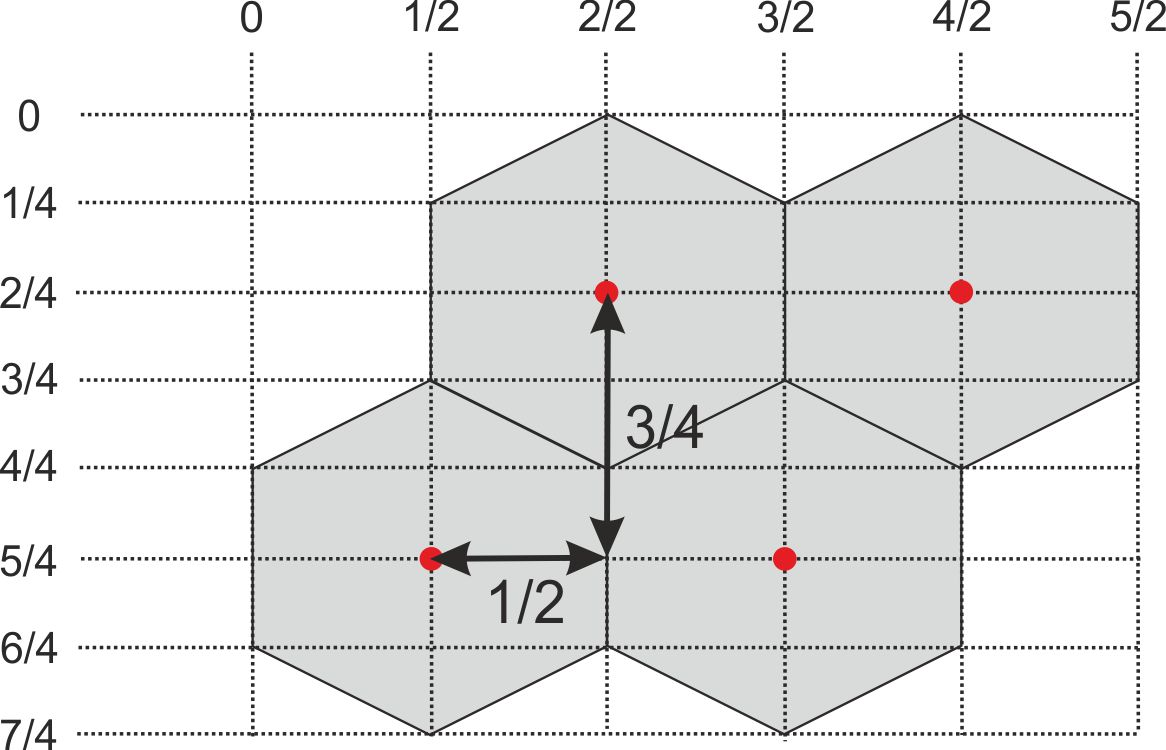
\includegraphics[scale=1.2]{kepek/PointyTop.jpg}
\caption{Felül hegyes elrendezés esetén az eltolások}
\label{fig:PointyTop}
\end{figure}

\begin{figure}[h!]
\centering
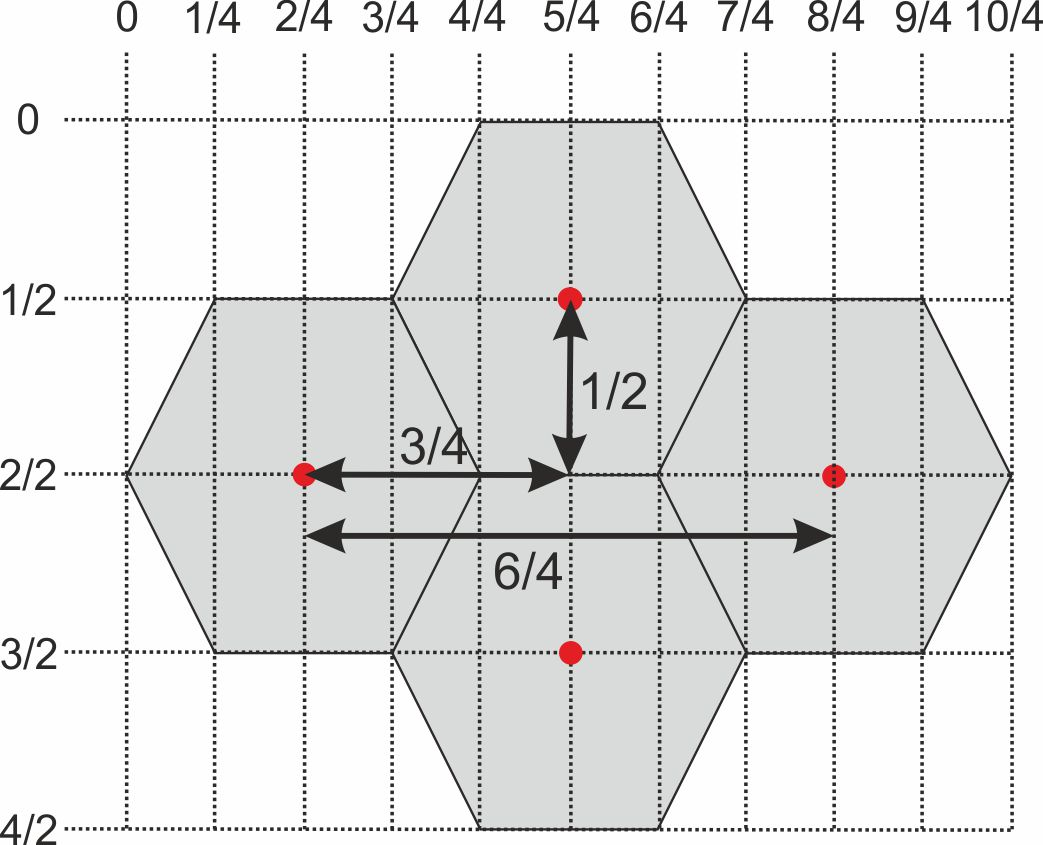
\includegraphics[scale=1.2]{kepek/FlatTop.jpg}
\caption{Felül lapos elrendezés esetén az eltolások}
\label{fig:FlatTop}
\end{figure}
